% Options for packages loaded elsewhere
\PassOptionsToPackage{unicode}{hyperref}
\PassOptionsToPackage{hyphens}{url}
\PassOptionsToPackage{dvipsnames,svgnames*,x11names*}{xcolor}
%
\documentclass[
  11pt,
]{article}
\usepackage{lmodern}
\usepackage{amssymb,amsmath}
\usepackage{ifxetex,ifluatex}
\ifnum 0\ifxetex 1\fi\ifluatex 1\fi=0 % if pdftex
  \usepackage[T1]{fontenc}
  \usepackage[utf8]{inputenc}
  \usepackage{textcomp} % provide euro and other symbols
\else % if luatex or xetex
  \usepackage{unicode-math}
  \defaultfontfeatures{Scale=MatchLowercase}
  \defaultfontfeatures[\rmfamily]{Ligatures=TeX,Scale=1}
\fi
% Use upquote if available, for straight quotes in verbatim environments
\IfFileExists{upquote.sty}{\usepackage{upquote}}{}
\IfFileExists{microtype.sty}{% use microtype if available
  \usepackage[]{microtype}
  \UseMicrotypeSet[protrusion]{basicmath} % disable protrusion for tt fonts
}{}
\makeatletter
\@ifundefined{KOMAClassName}{% if non-KOMA class
  \IfFileExists{parskip.sty}{%
    \usepackage{parskip}
  }{% else
    \setlength{\parindent}{0pt}
    \setlength{\parskip}{6pt plus 2pt minus 1pt}}
}{% if KOMA class
  \KOMAoptions{parskip=half}}
\makeatother
\usepackage{xcolor}
\IfFileExists{xurl.sty}{\usepackage{xurl}}{} % add URL line breaks if available
\IfFileExists{bookmark.sty}{\usepackage{bookmark}}{
\usepackage{hyperref}
}
\hypersetup{
  pdftitle={Cours sur les dictionnaires},
  pdfauthor={Première NSI, Lycée du Parc},
  colorlinks=true,
  linkcolor=Maroon,
  filecolor=Maroon,
  citecolor=Blue,
  urlcolor=Blue,
  pdfcreator={LaTeX via pandoc}}
\urlstyle{same} % disable monospaced font for URLs
\usepackage[top=20mm,left=20mm,right=20mm,heightrounded]{geometry}
\usepackage{listings}
\newcommand{\passthrough}[1]{#1}
\lstset{defaultdialect=[5.3]Lua}
\lstset{defaultdialect=[x86masm]Assembler}
\usepackage{graphicx}
\makeatletter
\def\maxwidth{\ifdim\Gin@nat@width>\linewidth\linewidth\else\Gin@nat@width\fi}
\def\maxheight{\ifdim\Gin@nat@height>\textheight\textheight\else\Gin@nat@height\fi}
\makeatother
% Scale images if necessary, so that they will not overflow the page
% margins by default, and it is still possible to overwrite the defaults
% using explicit options in \includegraphics[width, height, ...]{}
\setkeys{Gin}{width=\maxwidth,height=\maxheight,keepaspectratio}
% Set default figure placement to htbp
\makeatletter
\def\fps@figure{htbp}
\makeatother
\setlength{\emergencystretch}{3em} % prevent overfull lines
\providecommand{\tightlist}{%
  \setlength{\itemsep}{0pt}\setlength{\parskip}{0pt}}
\setcounter{secnumdepth}{5}

\title{Cours sur les dictionnaires}
\usepackage{etoolbox}
\makeatletter
\providecommand{\subtitle}[1]{% add subtitle to \maketitle
  \apptocmd{\@title}{\par {\large #1 \par}}{}{}
}
\makeatother
\subtitle{Thème types construits}
\author{Première NSI, \href{https://frederic-junier.org/}{Lycée du
Parc}}
\date{}

%%%jolis boites

\usepackage{fancybox, graphicx}



%%%%%%%%%%%%%%%%Packages et Macros Frederic%%%%%%%%%%%%%%%%%%%%%%%%%%%%%


%%%%Insertion de liens hypertextes %%%%

            
%%%%%%%%%%PSTricks%%%%%%%%%%%%

\usepackage{pstricks,pst-plot,pst-text,pst-tree,pst-eps,pst-fill,pst-node,pst-math,pstricks-add,pst-xkey,pst-eucl}


%%%%%%%Tikz%%%%%%%%%%%%%%%
\usepackage{pgf,tikz,tkz-tab}
% Pour les tableaux de signes ou de variations avec tkz-tab voir https://zestedesavoir.com/tutoriels/439/des-tableaux-de-variations-et-de-signes-avec-latex/#1-13389_tikz-un-package-qui-en-a-dans-le-ventre
\usetikzlibrary{arrows}
\usetikzlibrary{shapes.geometric}
\usetikzlibrary{shapes.geometric}
\usetikzlibrary{petri}
\usetikzlibrary{decorations}
\usetikzlibrary{arrows}
\usetikzlibrary{math}
 %Variables must be declared in a tikzmath environment but
       % can be used outside
%       \tikzmath{int \n; \n = 508; \x1 = 1; \y1 =1; 
%                   %computations are also possible
%                    \x2 = \x1 + 1; \y2 =\y1 +3; } 


%%%%%%%%%%%%%%%%%%%%%%%%%%%%%%%%%%%%%%%%
%%%%%%%%%%%Commandes Tikz Perso%%%%%%%%%%%%%%%

% Définition des nouvelles options xmin, xmax, ymin, ymax
% Valeurs par défaut : -3, 3, -3, 3
\tikzset{
xmin/.store in=\xmin, xmin/.default=-3, xmin=-3,
xmax/.store in=\xmax, xmax/.default=3, xmax=3,
ymin/.store in=\ymin, ymin/.default=-3, ymin=-3,
ymax/.store in=\ymax, ymax/.default=3, ymax=3,
}
% Commande qui trace la grille entre (xmin,ymin) et (xmax,ymax)
\newcommand {\grille}[2]
{\draw[help lines,black, thick] (\xmin,\ymin) grid[xstep=#1, ystep=#2] (\xmax,\ymax);}
% Commande \axes
\newcommand {\axes} {
\draw[->,very thick] (\xmin,0) -- (\xmax,0);
\draw[->,very thick] (0,\ymin) -- (0,\ymax);
\draw (0.95*\xmax, 0) node[above] {};
\draw (0, 0.95*\ymax) node[left] {};
}
% Commande qui limite l?affichage à (xmin,ymin) et (xmax,ymax)
\newcommand {\fenetre}
{\clip (\xmin,\ymin) rectangle (\xmax,\ymax);}

%Exemple d'utilisation

%\begin{center}
%\begin{tikzpicture} [xmin=-2,xmax=2,ymin=0,ymax=5]
%\grille{1} \axes \fenetre
%\draw plot[smooth] (\x,\x^2);
%\end{tikzpicture}
%\end{center}

%style pour la perspective cavalière française
%voir Tikz pour l'impatient page 68
\tikzset{math3d/.style=
{x= {(-0.353cm,-0.353cm)}, z={(0cm,1cm)},y={(1cm,0cm)}}}

%%%%%%%Symbole pour code calculatrice%%%%%%

%Flèche remplie pour défilement de menu

\newcommand{\flechefillright}{

\begin{tikzpicture}[scale=0.15] \fill (0,0)--(2,1)--(0,2)--cycle;
\end{tikzpicture}}

%%%%%%%%%%%%%Symboles pour calculatrice Casio%%%%
\newcommand{\execasio}{\Pisymbol{psy}{191}} %Retour chariot
\newcommand{\dispcasio}{\begin{pspicture}(.1,.1)\pspolygon*(.1,0)(.1,.1)\end{pspicture}} %Triangle « Disp »
\newcommand{\dispcasiotikz}{
\begin{tikzpicture}[scale=0.2]
\fill (0,0) -- (1,0) -- (1,1) -- cycle;
\end{tikzpicture}} %Triangle « Disp »
%

%Fleche entre deux lignes, d'apres 'un bon petit' : http://forum.mathematex.net/latex-f6/fleches-entre-deux-lignes-pour-resolution-d-equation-t10283.html#p99817
\newcommand\addnode[1]{\Rnode{#1}{}}
\newcommand\linknode[3]{\ncbar[angleA=0,angleB=0,nodesep=1ex,arm=10ex,offset=-2pt]{->}{#1}{#2}\Aput{\vphantom{x}#3}}


%%Commande pour touche de calculatrice

\newcommand\tc[1]{%
{
\begin{tikzpicture}
\node[draw,rectangle,rounded corners=3pt] (P) at (0,0){#1};
\end{tikzpicture}
}
}

%%%%%%%%%%%%%%%%%%%%%%%%%%%%%%%%%%%%%%%%
%%%%%%%%%%%Fin Commandes Tikz%%%%%%%%%%%%%%%


%%%%%%%%%%%%Specifiques%%%%%%%%%%%
\usepackage{wrapfig}
%pour insérer une figure à droite ou à gauche d'un texte
%\begin{wrapfigure}[nb lignes]{placement l,r,c,i(inside),o(outside)}[overhang]{width}
%ce package fonctionne mal à proximité des listes
%%%%%%%%%%%%%%%%%%%%%%%%%%%%%%%%%%%%%

%%%%%Environnements et symboles spéciaux pour faire joli%%%%%%

%%%Bclogo, pour des environnements + jolis avec insertion de logo%%%%
%Dépendances de  bclogo
\usepackage{xkeyval}  
\usepackage{etoolbox}
\usepackage{ifpdf}
\usepackage[framemethod=tikz]{mdframed}
\usepackage[tikz]{bclogo}

%\newcommand\bcpython{\includegraphics[width=17pt]{/home/fjunier/Maths/python-logo.eps}}
\newcommand\bcpython{\includegraphics[width=17pt]{/home/fjunier/Maths/python-logo.png}}
%\newcommand\bcpython{\includegraphics[width=17pt]{/home/frederic/Maths/python-logo.png}}

%% Framed
\usepackage{framed}  %Le package « framed» Crée 3 nouveaux environnements, qui se comportent comme des minipage de largeur \linewidth, mais permettant en plus de se casser entre plusieurs pages.     * framed : avec un cadre autour;     * shaded : avec un fonc coloré (il faut définir la couleur shadecolor);     * leftbar : avec une barre le long du côté gauche.

%%%%%%%%%%%%%%%%%%%Présentation de codes sources%%%%%%%%%%%%%%%%%
\usepackage{listings}
%On utilise l?environnement lstlisting pour insérer
%un code source.
%En plus de l?environnement lstlisting, on peut également utiliser la
%commande \lstinline qui fonctionne comme la commande \verb, en ce
%sens qu?on peut utiliser n?importe quel caractère comme délimiteur. Enfin,
%la commande \lstinputlisting permet de charger un code source depuis
%un fichier externe.
%Il y a deux manières de préciser des options : soit via l?option de l?envi-
%ronnement ou de la commande, soit en utilisant la commande \lstset
%qui permet de définir des options de manière globale.

\lstset{ %
  language=Python,                % the language of the code
  basicstyle=\ttfamily,           % the size of the fonts that are used for the code
  %numbers=left,                   % where to put the line-numbers
  numberstyle=\tiny,  % the style that is used for the line-numbers
  %stepnumber=2,                   % the step between two line-numbers. If it's 1, each line 
                                  % will be numbered
  %numbersep=5pt,                  % how far the line-numbers are from the code
  backgroundcolor=\color{white},      % choose the background color. You must add \usepackage{color}
  showspaces=false,               % show spaces adding particular underscores
  showstringspaces=false,         % underline spaces within strings
  showtabs=false,                 % show tabs within strings adding particular underscores
  frame=single,                   % adds a frame around the code
  rulecolor=\color{black},        % if not set, the frame-color may be changed on line-breaks within not-black text (e.g. comments (green here))
  tabsize=4,                      % sets default tabsize to 2 spaces
  captionpos=b,                   % sets the caption-position to bottom
  breaklines=true,                % sets automatic line breaking
  breakatwhitespace=false,        % sets if automatic breaks should only happen at whitespace
  %title=\lstname,                   % show the filename of files included with \lstinputlisting;
                                  % also try caption instead of title
  breakindent=1cm,
  keywordstyle=\color{blue},          % keyword style
  commentstyle=\color{red},       % comment style
  %stringstyle=\ttfamily\color{green},         % string literal style
  escapeinside={\%*}{*)},            % if you want to add LaTeX within your code
  morekeywords={*,...},              % if you want to add more keywords to the set
  deletekeywords={...}              % if you want to delete keywords from the given language
  upquote=true,columns=flexible,
xleftmargin=1cm,xrightmargin=1cm,
 inputencoding=utf8,			%Les lignes qui suivent sont pour le codage utf8
  extendedchars=true,
  literate=%
            {é}{{\'{e}}}1
            {è}{{\`{e}}}1
            {ê}{{\^{e}}}1
            {ë}{{\¨{e}}}1
            {û}{{\^{u}}}1
            {ù}{{\`{u}}}1
            {â}{{\^{a}}}1
            {à}{{\`{a} }}1
            {î}{{\^{i}}}1
            {ô}{{\^{o}}}1
            {ç}{{\c{c}}}1
            {Ç}{{\c{C}}}1
            {É}{{\'{E}}}1
            {Ê}{{\^{E}}}1
            {À}{{\`{A}}}1
            {Â}{{\^{A}}}1
            {Î}{{\^{I}}}1
}

\lstdefinestyle{rond}{
  numbers=none,
  backgroundcolor=\color{gristclair},
  frameround =tttt
}

\lstdefinestyle{compil}{
  numbers=none,
  backgroundcolor=\color{gristclair}
}
%\lstset{language=Python,basicstyle=\small , frame=single,tabsize=4,showspaces=false,showtabs=false,showstringspaces=false,numbers=left,numberstyle=\tiny , extendedchars=true}



%%%%%%%%%%%%%%%%%%%%%%%%%%%%%%%%%%%%%%%%%%%%%%%%%%%%%%%%%%%%%%%%%%%%%%%%
%%%%%%%%%%%%%%%%%%%%Environnements persos%%%%%%%%%%%%%%%%%%%%%%%%%%%%%%%%
%Syntaxe :
%\newenvironment{nom}[nombre d'args][defaut]{definitions initiales}{definitions finales}
%definitions intiales sont les commandes appelées par \begin{nom}
%Definitions finales sont les commandes appelées par \end{nom}

%%%%%%%%%%%%%%%%Définitions des environnemts persostheoreme, exemple ..%%%%
%%%% Exercice avec encadré %%%%
\newcounter{exo}
\newenvironment{exercice}[1]
{\par \medskip   \addtocounter{exo}{1} \noindent  
\begin{bclogo}[arrondi =0.1,   noborder = true, logo=\bccrayon, marge=4]{~\textbf{Exercice} \textbf{\theexo} {\itshape #1} }  \par}
{
\end{bclogo}
 \par \bigskip }

%%Axiomes, Theoremes, Propriété, Définition, Methode, Preuve


\newenvironment{axiome}[1]
{\par \medskip   \begin{leftbar} \noindent \underline{\textbf{Axiome}}\hspace{0.5cm}{\itshape #1}   \vspace*{10pt} \par }
{\end{leftbar}  \par \medskip }


\newcounter{thme}
\newenvironment{theoreme}[1]
{\par \medskip  \addtocounter{thme}{1} \noindent  
\begin{bclogo}[arrondi =0.1,  ombre = true, barre=none, logo=\bcbook, marge=4]{~\textbf{Théorème} \textbf{\thethme} {\itshape #1} }   \par}
{
\end{bclogo}
 \par \bigskip}

 \newenvironment{theoremedef}[1]
{\par \medskip   \addtocounter{thme}{1} \noindent  
\begin{bclogo}[arrondi =0.1,  ombre = true, barre=none, logo=\bcbook, marge=4]{~\textbf{Théorème-Définition} \textbf{\thethme} {\itshape #1} }   \par}
{
\end{bclogo}
 \par \bigskip }
 
\newcounter{prop}
\newenvironment{propriete}[1]
{\par \medskip   \addtocounter{prop}{1} \noindent  
\begin{bclogo}[arrondi =0.1,  ombre = true, barre=none, logo=\bcbook, marge=4]{~\textbf{Propriété} \textbf{\theprop} {\itshape #1} }   \par}
{
\end{bclogo}
 \par \bigskip }


\newenvironment{corollaire}[1]
{\par \medskip   \noindent  
\begin{bclogo}[arrondi =0.1,  ombre = true, barre=none, logo=\bcbook, marge=4]{~\textbf{Corollaire} {\itshape #1} } \par }
{
\end{bclogo}
 \par \bigskip }

\newenvironment{demo}[1]
{\par \medskip   \noindent  
\begin{bclogo}[arrondi =0.1,  ombre = true, barre=zigzag, noborder = true, logo=\bcloupe, marge=0]{~\textbf{Démonstration} {\itshape #1} } \par \vspace{10pt}}
{
\end{bclogo}
 \par \bigskip }

\newcounter{activite}
\newenvironment{activite}[1]
{\par \medskip   \noindent   \addtocounter{activite}{1}
\begin{bclogo}[arrondi =0.1,   noborder = true, logo=\bcvelo, marge=4]{~\textbf{Activité} \textbf{\theactivite} {\itshape #1} }  \par}
{
\end{bclogo}
 \par \bigskip }


\newenvironment{synthese}
{\par \medskip   \noindent   
\begin{bclogo}[arrondi =0.1,   noborder = true, logo=\bccle, marge=4]{~\textbf{Synthèse}   }  \par}
{
\end{bclogo}
 \par \bigskip }
 
 
\newcounter{rque}
\newenvironment{remarque}
{\par \medskip    \addtocounter{rque}{1} \noindent  
\begin{bclogo}[arrondi =0.1,  ombre = true, barre=snake, noborder = true, logo=\bcinfo, marge=0]{~\textbf{Remarque} \textbf{\therque}}  \par }
{
\end{bclogo}
 \par \bigskip }

\newcounter{def}
\newenvironment{definition}[1]
{\par \medskip   \addtocounter{def}{1} \noindent  
\begin{bclogo}[arrondi =0.1,  ombre = true, barre=none, logo=\bcbook, marge=4]{~\textbf{Définition} \textbf{\thedef} {\itshape #1} }  \par}
{
\end{bclogo}
 \par \bigskip }
 
 
 \newcounter{cours}
\newenvironment{cours}[1]
{\par \medskip   \addtocounter{cours}{1} \noindent  
\begin{bclogo}[arrondi =0.1,  ombre = true, barre=none, logo=\bcbook, marge=4]{~\textbf{Point de cours} \textbf{\thecours} {\itshape #1} }  \par}
{
\end{bclogo}
 \par \bigskip }
 
 

\newenvironment{introduction}
{\par \medskip    \noindent  
 \begin {bclogo}[couleur = blue!5 , arrondi =0.1,logo=\bcrosevents, marge=4] {~\textbf{Introduction}    }
 \par }
{
\end{bclogo}
 \par \bigskip }
 
\newenvironment{memo}[1]
{\par \medskip    \noindent  
\begin{bclogo}[arrondi =0.1,  ombre = true, barre=none, logo=\bccle, marge=4]{~\textbf{À retenir}  {\itshape #1} }  \par}
{
\end{bclogo}
 \par \bigskip }
 
\newcounter{exple}
\newenvironment{exemple}[1]
{\par \medskip   \addtocounter{exple}{1} \noindent  
\begin{bclogo}[arrondi =0.1,   noborder = true, logo=\bclampe, marge=4]{~\textbf{Exemple} \textbf{\theexple} {\itshape #1} }  \par}
{
\end{bclogo}
 \par \bigskip }




\newcounter{alg}
\newenvironment{algorithme}[1]
{\par \medskip   \addtocounter{alg}{1} \noindent  
 \begin {bclogo}[noborder = true, barre=zigzag,logo=\bcpython, marge=4] {~\textbf{Algorithmique} \textbf{\thealg} {\itshape #1} }  \par}
{
\end{bclogo}
 \par \bigskip }

\newcounter{prog}
\newenvironment{programme}[1]
{\par \medskip   \addtocounter{prog}{1} \noindent  
 \begin {bclogo}[noborder = true, barre=zigzag,logo=\bcpython, marge=4] {~\textbf{Programme} \textbf{\theprog} {\itshape #1} }  \par  \bigskip}
{
\end{bclogo}
 \par \bigskip }
 
\newcounter{logi}
\newenvironment{logique}[1]
{\par \medskip   \addtocounter{logi}{1} \noindent  
 \begin {bclogo}[noborder = true, barre=zigzag,logo=\bclampe, marge=4] {~\textbf{Logique} \textbf{\thelogi} {\itshape #1} }  \par}
{
\end{bclogo}
 \par \bigskip }


\newenvironment{methode}[1]
{\par \medskip    \noindent  
 \begin {bclogo}[arrondi =0.1,logo=\bcoutil, marge=4,noborder = true] {~\textbf{Méthode}   {\itshape #1} }  \par}
{
\end{bclogo}
 \par \bigskip }


\newcounter{histo}
\newenvironment{histoire}[1]
{\par \medskip   \addtocounter{histo}{1} \noindent  
 \begin {bclogo}[couleur = blue!10 , arrondi =0.1,logo=\bchorloge, marge=4] {~\textbf{Histoire} \textbf{\thehisto} {\itshape #1} }  \par}
{
\end{bclogo}
 \par \bigskip }




%Environnement contenu pour un document présentant une progression annuelle
\newenvironment{contenu}
{\par \medskip   \begin {bclogo}[ noborder = true,logo=\bccrayon] \noindent {\large \textbf{Contenu de la séance}} \vspace*{10pt} \par  }
{\end{bclogo}  \par \medskip }

%Environnement programme pour un document présentant une progression annuelle
%\newenvironment{programme}
%{\par \medskip   \begin {bclogo}[ noborder = true, barre=zigzag,logo=\bcinfo] \noindent {\large \textbf{Programme officiel}} \vspace*{10pt} \par  }
%{\end{bclogo}  \par \medskip }

%Environnement programme pour un document présentant une progression annuelle
\newenvironment{ressource}
{\par \medskip   \begin {bclogo}[ noborder = true,logo=\bcbook] \noindent {\large \textbf{Ressources}}\\vspace*{10pt} \par }
{\end{bclogo}  \par \medskip }




%%%%%%%%%%%%%%%%%%Maths divers%%%%%%%%%%%%%%%%%%%%%%%%%
%%%%%%%%%%%%%Nombres%%%%%%%%%%%%%%%%

%Ensemble prive de...
%\newcommand{\prive}{\boi}%{\backslash}

%Ensembles de nombres%%%%%%%%%%%%%%%%%
\newcommand{\R}{\mathbb{R}}
\newcommand{\N}{\mathbb{N}}
\newcommand{\D}{\mathbb{D}}
\newcommand{\Z}{\mathbb{Z}}
\newcommand{\Q}{\mathbb{Q}}
%\newcommand{\C}{\mathbb{C}}
\newcommand{\df}{~\ensuremath{]0;+\infty[}~}
\newcommand{\K}{\mathbb{K}}

%%%%%%%%Arithmetique%%%%%%%%%%
%PGCD, PPCM
\newcommand{\PGCD}{\mathop{\rm PGCD}\nolimits}
\newcommand{\PPCM}{\mathop{\rm PPCM}\nolimits}

%Intervalles
\newcommand{\interoo}[2]{]#1\, ;\, #2[}
\newcommand{\Interoo}[2]{\left]#1\, ;\, #2\right[}
\newcommand{\interof}[2]{]#1\, ;\, #2]}
\newcommand{\Interof}[2]{\left]#1\, ;\, #2\right]}
\newcommand{\interfo}[2]{[#1\, ;\, #2[}
\newcommand{\Interfo}[2]{\left[#1\, ;\, #2\right[}
\newcommand{\interff}[2]{[#1\, ;\, #2]}
\newcommand{\Interff}[2]{\left[#1\, ;\, #2\right]}
%\newcommand\interentiers #1#2{[\! [#1\, ;\, #2]\! ]}
\newcommand{\interentiers}[2]{\llbracket #1\, ;\, #2\rrbracket}
%


%%%%%%%%%%%%%%Nombres complexes%%%%%

\newcommand{\ic}{\text{i}}
%\newcommand{\I}{\text{i}}
\newcommand{\im}[1]{\text{Im}\left(#1\right)}
\newcommand{\re}[1]{\text{Re}\left(#1\right)}
\newcommand{\Arg}[1]{\text{arg}\left(#1\right)}
\newcommand{\Mod}[1]{\left[#1\right]}
%Parties entière, réelle, imaginaire, nombre i
\newcommand{\ent}[1]{\text{E}\left(#1\right)}
\renewcommand{\Re}{\mathop{\rm Re}\nolimits}
\renewcommand{\Im}{\mathop{\rm Im}\nolimits}
\renewcommand{\i}{\textrm{i}}

%%%%%%%%%%%Probabilites et statistiques%%%%%
\newcommand{\loibinom}[2]{\mathcal{B}\left(#1\ ; \ #2 \right)}
\newcommand{\loinorm}[2]{\mathcal{N}\left(#1\ ; \ #2 \right)}
\newcommand{\loiexp}[1]{\mathcal{E}\left(#1\right)}
\newcommand{\proba}[1]{\mathbb{P}\big(#1\big)}
\newcommand{\probacond}[2]{\mathbb{P}_{#2}\big(#1\big)}
\newcommand{\esperance}[1]{\mathbb{E}\left(#1\right)}
\newcommand{\variance}[1]{\mathbb{V}\left(#1\right)}
\newcommand{\ecart}[1]{\sigma\left(#1\right)}
\newcommand{\dnormx}{\frac{1}{\sqrt{2\pi}} \text{e}^{-\frac{x^2}{2}}}
\newcommand{\dnormt}{\frac{1}{\sqrt{2\pi}} \text{e}^{-\frac{t^2}{2}}}

%Covariance
\newcommand{\cov}{\mathop{\rm cov}\nolimits}
%


%%%%%%%%%%Analyse%%%%%%%%%%%

%%%%%%%%%%%Courbe%%%%%%%%%%%%
\newcommand{\courbe}[1]{\ensuremath{\mathcal{C}_{#1}}}

%%%%%%%Fonction exponentielle%%%%%
\newcommand{\fe}{~fonction exponentielle~}
\newcommand{\e}{\text{e}}

%Fonction cotangente
\newcommand{\cotan}{\mathop{\rm cotan}\nolimits}
%%%%%%%%%%%%%%%%%%%%%%%%%%%%%%%%%%%%%%%%%
%
%Fonctions hyperboliques
\newcommand{\ch}{\mathop{\rm ch}\nolimits}
\newcommand{\sh}{\mathop{\rm sh}\nolimits}


%%%%%%%%%%%%%%Limites%%%%%%
\newcommand{\limite}[2]{\lim\limits
_{x \to #1} #2}
\newcommand{\limitesuite}[1]{\lim\limits
_{n \to +\infty} #1}
\newcommand{\limiteg}[2]{\lim\limits
_{\substack{x \to #1 \\ x < #1 }} #2}
\newcommand{\limited}[2]{\lim\limits
_{\substack{x \to #1 \\ x > #1 }} #2}

%%%%%%%%%%Continuité%%%%%%%%%%%
\newcommand{\TVI}{théorème des valeurs intermédiaires}

%%%%%%%%%%%Suites%%%%%%%%%%%%
\newcommand{\suite}[1]{\ensuremath{\left(#1_{n}\right)}}
\newcommand{\Suite}[2]{\ensuremath{\left(#1\right)_{#2}}}
%

%%%%%%%%%%%%%%%Calcul intégral%%%%%%
\newcommand{\dx}{\ensuremath{\text{d}x}}		% dx
\newcommand{\dt}{\ensuremath{\text{d}t}}		% dt
\newcommand{\dtheta}{\ensuremath{\text{d}\theta}}		% dtheta
\newcommand{\dy}{\ensuremath{\text{d}y}}		% dy
\newcommand{\dq}{\ensuremath{\text{d}q}}		% dq

%%%Intégrale%%%
\newcommand{\integralex}[3]{\int_{#1}^{#2} #3 \ \dx}
\newcommand{\integralet}[3]{\int_{#1}^{#2} #3 \ \dt}
\newcommand{\integraletheta}[3]{\int_{#1}^{#2} #3 \ \dtheta}

%%%%%Equivalent%%
\newcommand{\equivalent}[1]{\build\sim_{#1}^{}}

%o et O%%%%
\renewcommand{\o}[2]{\build o_{#1\to #2}^{}}
\renewcommand{\O}[2]{\build O_{#1\to #2}^{}}



%%%%%%%%%%%%%%%Geometrie%%%%%%%%%%%%%%%%%%%%%%%

%%%%%%%%%%%%%%%Reperes%%%%%%%%%%%%%%
\def\Oij{\ensuremath{\left(\text{O},~\vect{\imath},~\vect{\jmath}\right)}}
\def\Oijk{\ensuremath{\left(\text{O},~\vect{\imath},~ \vect{\jmath},~ \vect{k}\right)}}
\def\Ouv{\ensuremath{\left(\text{O},~\vect{u},~\vect{v}\right)}}
\renewcommand{\ij}{(\vec\imath\, ;\vec\jmath\,)}
\newcommand{\ijk}{(\vec\imath\, ;\vec\jmath\, ;\vec k\,)}
\newcommand{\OIJ}{(O\,;\, I\,;\, J\,)}
\newcommand{\repere}[3]{\big(#1\, ;\,\vect{#2} ;\vect{#3}\big)}
\newcommand{\reperesp}[4]{\big(#1\, ;\,\vect{#2} ;\vect{#3} ;\vect{#4}\big)}

%%%%%%%%%Coordonnees%%%%%%%%%%%%%%
\newcommand{\coord}[2]{(#1\, ;\, #2)}
\newcommand{\bigcoord}[2]{\big(#1\, ;\, #2\big)}
\newcommand{\Coord}[2]{\left(#1\, ;\, #2\right)}
\newcommand{\coordesp}[3]{(#1\, ;\, #2\, ;\, #3)}
\newcommand{\bigcoordesp}[3]{\big(#1\, ;\, #2\, ;\, #3\big)}
\newcommand{\Coordesp}[3]{\left(#1\, ;\, #2\, ;\, #3\right)}
\newcommand{\Vcoord}[3]{\begin{pmatrix} #1 \\ #2 \\ #3 \end{pmatrix}}
%Symboles entre droites
%\newcommand{\paral}{\sslash}
\newcommand{\paral}{\mathop{/\!\! /}}
%

%%%%%%%%%Produit scalaire, Angles%%%%%%%%%%
\newcommand{\scal}[2]{\vect{#1} \, \cdot \, \vect{#2}}
\newcommand{\Angle}[2]{\left(\vect{#1} \, , \, \vect{#2}\right)}
\newcommand{\Anglegeo}[2]{\left(\widehat{\vect{#1} \, ; \, \vect{#2}}\right)}
\renewcommand{\angle}[1]{\widehat{#1}}
\newcommand{\anglevec}[2]{\left(\vect {#1}\, ,\,\vect {#2} \right)}
\newcommand{\anglevecteur}[2]{(#1\, , \, #2)}
\newcommand{\Anglevec}[2]{(\vecteur{#1}\, ,\,\vecteur{#2})}
\newcommand{\prodscal}[2]{#1 \, \cdot \, #2}
%


%Arc
%\newcommand{\arc}[1]{\wideparen{#1}}
\newcommand{\arcoriente}[1]{\overset{\curvearrowright}{#1}}
%
%


%%%%%%%%%%%%%%%Normes%%%%%%%%%%%%%%%%
\newcommand{\norme}[1]{\left\| #1\right\|}
\newcommand{\normebis}[1]{\delim{2pt}{\|}{9pt}\! #1\delim{2pt}{\|}{9pt}}
\newcommand{\normetriple}[1]{\left |\kern -.07em\left\| #1\right |\kern -.07em\right\|}
\newcommand{\valabs}[1]{\big| \, #1 \, \big|}
%

%%%%%%%%%%%%%%%%%%%%%%%%%%%Degré%%%%%%
%\newcommand{\Degre}{\ensuremath{^\circ}}
%La commande \degre est déjà définie dans le package babel

%%%%%%%%%%Vecteurs%%%%%%%%%%%
\newcommand{\vect}[1]{\mathchoice%
{\overrightarrow{\displaystyle\mathstrut#1\,\,}}%
{\overrightarrow{\textstyle\mathstrut#1\,\,}}%
{\overrightarrow{\scriptstyle\mathstrut#1\,\,}}%
{\overrightarrow{\scriptscriptstyle\mathstrut#1\,\,}}}



%%%%%%%%%%%%%Algebre%%%%%%%%%%%%%%%


%%%%%%%%%%Systemes%%%%%%%%%%%
%Systemes
\newcommand{\sys}[2]{
\left\lbrace
 \begin{array}{l}
  \negthickspace\negthickspace #1\\
  \negthickspace\negthickspace #2\\
 \end{array}
\right.\negthickspace\negthickspace}
\newcommand{\Sys}[3]{
\left\lbrace
 \begin{array}{l}
  #1\\
  #2\\
  #3\\
 \end{array}
\right.}
\newcommand{\Sysq}[4]{
\left\lbrace
 \begin{array}{l}
  #1\\
  #2\\
  #3\\
  #4\\
 \end{array}
\right.}
%
%

%%%%%%%%%%%%%%%%Matrices%%%%%%%%%%%%%%%%%%
%Comatrice
\newcommand{\com}{\mathop{\rm com}\nolimits}
%
%
%Trace
\newcommand{\tr}{\mathop{\rm tr}\nolimits}
%
%
%Transposee
\newcommand{\transposee}[1]{{\vphantom{#1}}^t\negmedspace #1}
%
%
%Noyau
\newcommand{\Ker}{\mathop{\rm Ker}\nolimits}
%
%

%
%Matrices
\newcommand{\Mn}{\mathcal M_n}
\newcommand{\matrice}[4]{
\left(
 \begin{array}{cc}
  #1 & #2 \\
  #3 & #4
 \end{array}
\right)}

\newcommand{\Matrice}[9]{
\left(
 \begin{array}{ccc}
  #1 & #2 & #3\\
  #4 & #5 & #6\\
  #7 & #8 & #9
 \end{array}
\right)}
\newcommand{\Vect}[3]{
\left(\negmedspace
 \begin{array}{c}
  #1\\
  #2\\
  #3
 \end{array}\negmedspace
\right)}
\newcommand{\Ideux}{\matrice{1}{0}{0}{1}}
\newcommand{\Itrois}{\Matrice{1}{0}{0}{0}{1}{0}{0}{0}{1}}
%
%
%Determinants
\newcommand{\determinant}[4]{
\left|
 \begin{array}{cc}
  #1 & #2 \\
  #3 & #4
 \end{array}
\right|}
\newcommand{\Determinant}[9]{
\left|
 \begin{array}{ccc}
  #1 & #2 & #3\\
  #4 & #5 & #6\\
  #7 & #8 & #9
 \end{array}
\right|}

\begin{document}
\maketitle

\renewcommand*\contentsname{Table des matières}
{
\hypersetup{linkcolor=}
\setcounter{tocdepth}{3}
\tableofcontents
}
\hypertarget{cruxe9dits}{%
\section*{Crédits}\label{cruxe9dits}}
\addcontentsline{toc}{section}{Crédits}

\emph{Ce cours est inspiré du chapitre 14 du manuel NSI de la collection
Tortue chez Ellipse, auteurs : Ballabonski, Conchon, Filliatre, N'Guyen.
J'ai également consulté le prepabac Première NSI de Guillaume Connan
chez Hatier, le
\href{https://cache.media.eduscol.education.fr/file/NSI/77/7/RA_Lycee_G_NSI_repd_types_construits_1170777.pdf}{document
ressource eduscol sur les types construits} et le livre \textbf{Fluent
Python}.}

\emph{Tous les exemples du cours peuvent être testés dans le fichier
\url{exemples_cours_dictionnaires_eleves.py}.}

\hypertarget{p-uplets-nommuxe9s-et-dictionnaires}{%
\section{\texorpdfstring{\texttt{p-uplets} nommés et
dictionnaires}{p-uplets nommés et dictionnaires}}\label{p-uplets-nommuxe9s-et-dictionnaires}}

\begin{exemple}{}

Dans le TP sur les \textbf{p-uplets} (nommés aussi \textbf{tuples}) on a
travaillé sur un fichier \passthrough{\lstinline!airports-reduit.csv!}
qui contient les enregistrements
\passthrough{\lstinline!nom;latitude;longitude;altitude;code\_pays!}
pour 57302 aéroports et on a extrait cette série dans un tableau de
\textbf{tuples}. Par exemple le \textbf{tuple} correspondant à
l'aéroport Saint-Exupéry est :

\begin{lstlisting}[language=Python]
>>> p_uplet = tab_tuple_airports[32478]
>>> p_uplet
('Lyon Saint-Exupéry Airport', '45.725556', '5.081111', '821', 'FR')
>>> p_uplet[1]
'45.725556'
\end{lstlisting}

Pour traiter cette information, il faut connaître la signification de
chaque élément (appelé aussi \emph{champ}) du \textbf{tuple} puisqu'on y
accède par son index entier : 0 pour le `nom', 1 pour la latitude etc
\ldots.

Il serait plus lisible de disposer d'un \textbf{tuple} à \emph{champs
nommés} et de pouvoir accéder à la valeur d'un champ par son nom. C'est
le dernier \textbf{type construit} de données que nous allons étudier.

\begin{lstlisting}[language=Python]
>>> p_uplet_nomme = tab_dico_airports[32478]
>>> p_uplet_nomme
{'nom': 'Lyon Saint-Exupéry Airport', 'latitude': '45.725556', 'longitude': '5.081111', 'altitude': '821', 'code_pays': 'FR'}
>>> p_uplet_nomme['latitude']
'45.725556'
\end{lstlisting}

\end{exemple}

\begin{definition}{}

Un \textbf{p-uplet nommé} (ou \textbf{tuple nommé}) est un
\textbf{p-uplet} dont chaque \textbf{élément} (ou \textbf{champ}) est
repéré par un nom et non par un entier. Ces \textbf{noms} sont appelés
\textbf{clefs} ou \textbf{descripteurs} du \textbf{p-uplet nommé}.
Celui-ci s'écrit entre accolades avec une virgule séparant chaque paire
constituée de la clef et de la valeur de la composante séparées par le
symbole \passthrough{\lstinline!:!}.

En
\href{https://docs.python.org/3/tutorial/datastructures.html}{Python},
les \textbf{p-uplets nommés} sont implémentés par les
\textbf{dictionnaires} de type \passthrough{\lstinline!dict!}. Par la
suite nous parlerons de \textbf{dictionnaire} plutôt que de
\textbf{p-uplet nommé}.

Comme l'accès aux valeurs s'effectue par les noms/clefs, comme dans un
dictionnaire où chaque nom est associé à sa définition, on parle aussi
de \textbf{tableaux associatifs}.

Un dictionnaire n'est pas une séquence ordonnée d'éléments, l'accès
s'effectue uniquement par clef.

\begin{lstlisting}[language=Python]
>>> python = {'apparition' : 1993, 'version' : '3.8', 'createur' : 'Guido Van Rossum'}
>>> python['createur']
'Guido Van Rossum'
>>> len(python)
3
>>> python[2]
Traceback (most recent call last):
  File "<stdin>", line 1, in <module>
KeyError: 2
\end{lstlisting}

\end{definition}

\hypertarget{un-exemple-de-dictionnaire-les-metadonnuxe9es-exif-dune-photo-numuxe9rique}{%
\section{Un exemple de dictionnaire : les metadonnées EXIF d'une photo
numérique}\label{un-exemple-de-dictionnaire-les-metadonnuxe9es-exif-dune-photo-numuxe9rique}}

Les photos prises avec un appareil numérique contiennent de nombreuses
informations. Dans un fichier image, par exemple au format
\passthrough{\lstinline!jpeg!}, sont stockées des données non seulement
sur l'image elle-même mais aussi des \textbf{metadonnées} sur
l'appareil, le logiciel utilisé, et en particulier des données
\href{https://fr.wikipedia.org/wiki/Exchangeable_image_file_format}{EXIF}
(Exchangeable Image File Format). Une partie est accessible dans les
propriétés de fichier ou avec un logiciel de traitement d'images. Les
spécifications sont gérées par un organisme japonais, le JEITA, qui
définit différents dictionnaires de référence permettant d'accéder à ces
données. Les clés (les tags) et les valeurs sont des nombres écrits dans
l'entête du fichier. Les dictionnaires donnent l'interprétation de ces
clés. Par exemple la clé 256 a pour valeur `Width' , la largeur de
l'image en pixel et la clé 257 a pour valeur `Length' , la hauteur de
l'image en pixel.

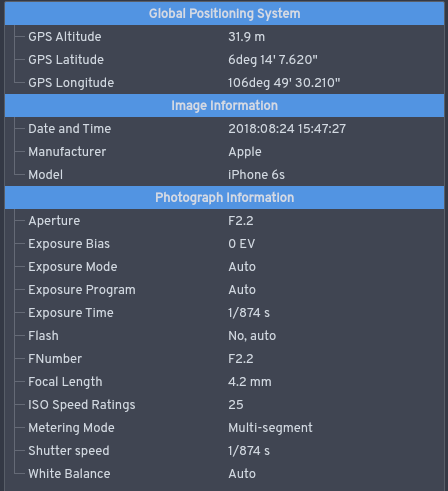
\includegraphics[width=0.5\textwidth,height=\textheight]{images/exif.png}\\

\emph{Source :
\url{https://commons.wikimedia.org/wiki/File:DigiKam_EXIF_information_screenshot.png}}

\begin{exercice}{}

On peut extraite les données EXIF avec le logiciel
\href{https://exiftool.org/}{exiftool}, le plugin Firefox
\href{https://addons.mozilla.org/fr/firefox/addon/exif-viewer/}{exifviewer}
ou sous forme de dictionnaire
\href{https://docs.python.org/3/tutorial/datastructures.html}{Python}
avec le module
\href{https://smarnach.githeub.io/pyexiftool/}{pyexiftool}. Le script
Python \passthrough{\lstinline!exiftool\_test.py!} ci-dessous contient
une fonction qui extrait les données
\href{https://fr.wikipedia.org/wiki/Exchangeable_image_file_format}{EXIF}
d'un fichier image passé en paramètre, sous la forme de dictionnaire.

\begin{lstlisting}[language=Python]
#!/usr/bin/env python3
# -*- coding: utf-8 -*-
import sys
import exiftool

def extraire_exif(fichier):
    et = exiftool.ExifTool()
    et.start()
    metadata = et.get_metadata(fichier)
    et.terminate()
    return metadata

#code client exécuté si script exécuté directement
if __name__ == "__main__": 
    #extrait les données exif du fichier passé en paramètre
    print(extraire_exif(sys.argv[1]))
\end{lstlisting}

\begin{enumerate}
\def\labelenumi{\arabic{enumi}.}
\tightlist
\item
  Télécharger la photo
  \url{http://frederic-junier.org/SNT/images/20181230_162625.jpg}.
\item
  Extraire ses données
  \href{https://fr.wikipedia.org/wiki/Exchangeable_image_file_format}{EXIF}
  avec \href{https://exiftool.org/}{exiftool} ou le script
  \href{https://docs.python.org/3/tutorial/datastructures.html}{Python},
  puis retrouver la commune où elle a été prise. Voici une partie du
  dictionnaire obtenu :
\end{enumerate}

\begin{lstlisting}[language=Python]
fjunier@fjunier:~/sandbox$ sudo apt install libimage-exiftool-perl
fjunier@fjunier:~/sandbox$ pip3 install --user pyexiftool
fjunier@fjunier:~/sandbox$ chmod +x exiftool_test.py 
fjunier@fjunier:~/sandbox$ ls -l exiftool_test.py 
-rwxrwxr-x 1 fjunier fjunier 355 févr. 24 21:50 exiftool_test.py
fjunier@fjunier:~/sandbox$ ./exiftool_test.py image_mystere.jpg 
{..., 'EXIF:Make': 'samsung', 'EXIF:Model': 'SM-G930F', 'EXIF:Orientation': 1, 'EXIF:XResolution': 72,
 'EXIF:YResolution': 72, 'EXIF:ResolutionUnit': 2, 'EXIF:Software': 'G930FXXU3ERL3', 'EXIF:ModifyDate': '2018:12:30 16:26:24', 'EXIF:YCbCrPositioning': 1, 'EXIF:ExposureTime': 0.0005733944954, 'EXIF:FNumber': 1.7, 'EXIF:ExposureProgram': 2, 'EXIF:ISO': 50,
 'EXIF:ExifVersion': '0220', 'EXIF:DateTimeOriginal': '2018:12:30 16:26:24', 'EXIF:CreateDate': '2018:12:30 16:26:24', 'EXIF:ComponentsConfiguration': '1 2 3 0', 'EXIF:ShutterSpeedValue': '0.000572673315054629', 'EXIF:ApertureValue': 1.6993699982773, 'EXIF:BrightnessValue': 8.36,
 'EXIF:ExposureCompensation': 0, 'EXIF:MaxApertureValue': 1.6993699982773, 'EXIF:MeteringMode': 2,
 'EXIF:Flash': 0, 'EXIF:FocalLength': 4.2, 'EXIF:UserComment': '', 'EXIF:SubSecTime': '0999',
 ...., 'EXIF:FlashpixVersion': '0100', 'EXIF:ColorSpace': 1, 'EXIF:ExifImageWidth': 4032, 'EXIF:ExifImageHeight': 3024, ..., 'EXIF:GPSVersionID': '2 2 0 0', 'EXIF:GPSLatitudeRef': 'N',
 'EXIF:GPSLatitude': 42.4947222222222, 'EXIF:GPSLongitudeRef': 'E', 'EXIF:GPSLongitude': 3.13,
 'EXIF:GPSAltitudeRef': 0, 'EXIF:GPSAltitude': 123, 'EXIF:GPSTimeStamp': '15:26:35','EXIF:GPSDateStamp': '2018:12:30', ....
 }
\end{lstlisting}

\end{exercice}

\hypertarget{cruxe9ation-de-dictionnaire}{%
\section{Création de dictionnaire}\label{cruxe9ation-de-dictionnaire}}

\begin{methode}{}

Il existe plusieurs façons de construire un dictionnaire :

\begin{itemize}
\tightlist
\item
  \textbf{Par extension :} On peut utiliser la forme littérale avec les
  accolades \passthrough{\lstinline!\{!} et \passthrough{\lstinline!\}!}
  qui entourent la série des paires
  \passthrough{\lstinline!clef : valeur!} ou le constructeur
  \passthrough{\lstinline!dict!} qui peut convertir en dictionnaire une
  séquence de \passthrough{\lstinline!tuple!} de la forme
  \passthrough{\lstinline!(clef, valeur)!}.
\end{itemize}

\begin{lstlisting}[language=Python]
>>> processeur1 = {'annee' : 1974, 'fabricant' : 'Intel', 'Frequence' : '2 MHz','gravure' : '6000 nm', 'architecture' : '8080'}
>>> processeur2 = dict([('annee', 1978), ('fabricant', 'Intel'),('Frequence','5 MHz'),('gravure','3 micrometres'),('architecture','8086')])
>>> processeur2
{'annee': 1978, 'fabricant': 'Intel', 'Frequence': '5 MHz', 'gravure': '3000 nm', 'architecture': '8086'}
>>> processeur1['gravure']
'6000 nm'
>>> processeur2['gravure']
'3000 nm'
\end{lstlisting}

\begin{itemize}
\tightlist
\item
  \textbf{Par compréhension :} La syntaxe est la même que pour les
  tableaux de type \passthrough{\lstinline!list!} en remplaçant les
  parenthèses par des accolades. On peut récupérer les paires
  \passthrough{\lstinline!clef : valeur!} en parcourant un tableau de
  \passthrough{\lstinline!tuple!}.
\end{itemize}

\begin{lstlisting}[language=Python]
>>> tab_tuple = [('annee', 1989), ('fabricant', 'Intel'),('Frequence','25 MHz'),('gravure','600 nm'),('architecture','80486')]
>>> processeur3 = { clef : valeur for clef, valeur in tab_tuple }
>>> processeur3
{'annee': 1989, 'fabricant': 'Intel', 'Frequence': '25 MHz', 'gravure': '600 nm', 'architecture': '80486'}
\end{lstlisting}

\end{methode}

\begin{exercice}{}

La fonction \passthrough{\lstinline!ord!} associe à un caractère son
point de code \href{https://fr.wikipedia.org/wiki/Unicode}{Unicode} et
sa réciproque est la fonction \passthrough{\lstinline!chr!}.

\begin{lstlisting}[language=Python]
>>> ord('a'), chr(97)
(97, 'a')
>>> [chr(k) for k in range(97, 97 + 10)]
['a', 'b', 'c', 'd', 'e', 'f', 'g', 'h', 'i', 'j']
\end{lstlisting}

Donner des expressions qui permettent de définir les dictionnaires
ci-dessous par compréhension :

\begin{lstlisting}[language=Python]
>>> ordinal
{'a': 97, 'b': 98, 'c': 99, 'd': 100, 'e': 101, 'f': 102, 'g': 103, 'h': 104, 'i': 105, 'j': 106}
>>> caractere
{97: 'a', 98: 'b', 99: 'c', 100: 'd', 101: 'e', 102: 'f', 103: 'g', 104: 'h', 105: 'i', 106: 'j'}
\end{lstlisting}

\end{exercice}

\hypertarget{accuxe8s-ajout-suppression-duxe9luxe9ment-dans-un-dictionnaire}{%
\section{Accès, ajout, suppression d'élément dans un
dictionnaire}\label{accuxe8s-ajout-suppression-duxe9luxe9ment-dans-un-dictionnaire}}

\begin{methode}{}

\begin{itemize}
\tightlist
\item
  L'accès, la modification, l'ajout d'un élément se fait avec
  l'opérateur crochet : \passthrough{\lstinline!dico[clef]!} renvoie la
  valeur appairée avec la clef donnée dans le dictionnaire
  \passthrough{\lstinline!dico!}. Le nombre d'éléments est donné par la
  fonction \passthrough{\lstinline!len!}, mais les éléments sont indexés
  par les clefs et non par des entiers : \emph{il n'y a pas de notion
  d'ordre dans un dictionnaire.} Comme les tableaux de type
  \passthrough{\lstinline!list!} et contrairement aux \textbf{p-uplets}
  de type \passthrough{\lstinline!tuple!}, les dictionnaires de type
  \passthrough{\lstinline!dict!} sont modifiables après modification ,
  on dit qu'ils sont \textbf{mutables}. Un dictionnaire peut être
  construit par ajout successif de paires
  \passthrough{\lstinline!clef : valeur!} à partir du dictionnaire vide
  \passthrough{\lstinline!\{\}!}. Enfin, on peut supprimer un élément si
  on connaît sa \passthrough{\lstinline!clef!} avec
  \passthrough{\lstinline!del dico[clef]!}.
\end{itemize}

\begin{lstlisting}[language=Python]
>>> nobel2019 = {}
>>> nobel2019['Littérature'] = 'Peter Handke'
>>> nobel2019
{'Littérature': 'Peter Handke'}
>>> nobel2019['Paix'] = 'Kim Joon Hyun'
>>> nobel2019
{'Littérature': 'Peter Handke', 'Paix': 'Kim Joon Hyun'}
>>> nobel2019['Paix'] = 'Abiy Ahmed'
>>> nobel2019
{'Littérature': 'Peter Handke', 'Paix': 'Abiy Ahmed'}
>>> nobel2019['Maths'] = 'Cédric Villani'
>>> nobel2019
{'Littérature': 'Peter Handke', 'Paix': 'Abiy Ahmed', 'Maths': 'Cédric Villani'}
>>> del nobel2019['Maths']
>>> nobel2019
{'Littérature': 'Peter Handke', 'Paix': 'Abiy Ahmed'}
\end{lstlisting}

\begin{itemize}
\tightlist
\item
  Parce qu'un dictionnaire est implémenté par une
  \href{https://fr.wikipedia.org/wiki/Table_de_hachage}{table de
  hachage}, ses \textbf{clefs} doivent, nécessairement être
  \textbf{immutables} (plus précisément récursivement immutables s'il
  s'agit de structures imbriquées et encore plus précisément
  \href{https://docs.python.org/3/glossary.html}{hachables}). Une valeur
  est \textbf{immutable} si elle ne peut pas être modifiée après sa
  création. Les types de base \passthrough{\lstinline!int!},
  \passthrough{\lstinline!float!}, \passthrough{\lstinline!bool!} et les
  types construits \passthrough{\lstinline!tuple!},
  \passthrough{\lstinline!str!} sont \textbf{immutables} mais pas les
  types \passthrough{\lstinline!list!} et \passthrough{\lstinline!dict!}
  (un dictionnaire ne peut pas être une clef de dictionnaire).
\end{itemize}

\begin{lstlisting}[language=Python]
>>> jouet =dict()
>>> jouet[2] = 'clef de type int'
>>> jouet[True] = 'clef de type bool'
>>> jouet[(1,2)] = 'clef de type tuple'
>>> jouet
{2: 'clef de type int', True: 'clef de type bool', (1, 2): 'clef de type tuple'}
>>> jouet[[1,2]] = 'clef de type list -> impossible'
Traceback (most recent call last):
  File "<stdin>", line 1, in <module>
TypeError: unhashable type: 'list'
\end{lstlisting}

\begin{itemize}
\tightlist
\item
  Une dictionnaire ne peut pas être une clef, mais peut être une valeur
  dans un autre dictionnaire. On peut définir toutes sortes de
  \textbf{structures imbriquées} comme des tableaux de dictionnaires
  \ldots{}
\end{itemize}

\begin{lstlisting}[language=Python]
>>> vols = {'Lisbonne': {'heure': '21:10','num': 'EJU7674','compagnie': 'EASYJET'},
... 'Vienne': {'heure': '21:25','num': 'OS430','compagnie': 'AUSTRIAN AIRLINES'},
... 'Londres': {'heure': '21:55','num': 'BA357','compagnie': 'BRITISH AIRWAYS'}}
>>> vols['Londres']
{'heure': '21:55', 'num': 'BA357', 'compagnie': 'BRITISH AIRWAYS'}
>>> tab_dico_airports
[{'nom': 'Total Rf Heliport','latitude': '40.07080078125', 'longitude': '-74.93360137939453',
  'altitude': '11',  'code_pays': 'US'},
   {'nom': 'Aero B Ranch Airport',  'latitude': '38.704022',  'longitude': '-101.473911',
  'altitude': '3435',  'code_pays': 'US'}]
\end{lstlisting}

\begin{itemize}
\tightlist
\item
  Avec l'opérateur crochet, si une clef n'appartient pas à un
  dictionnaire, une exception (erreur en
  \href{https://docs.python.org/3/tutorial/datastructures.html}{Python})
  est levée. La méthode \passthrough{\lstinline!get!} permet de
  retourner la valeur \passthrough{\lstinline!None!} par défaut si on ne
  veut pas d'erreur.
\end{itemize}

\begin{lstlisting}[language=Python]
>>> prix_turing2006 = {'nom' : 'Frances Allen', 'sujet' : 'Optimisation des compilateurs'}
>>> prix_turing2006['pays']
Traceback (most recent call last):
  File "<stdin>", line 1, in <module>
KeyError: 'pays'
>>> prix_turing2006.get('pays')
\end{lstlisting}

\end{methode}

\begin{exercice}{}

\emph{QCM de type E3C 2}.

\begin{enumerate}
\def\labelenumi{\arabic{enumi}.}
\tightlist
\item
  \textbf{Question 1} Comment peut-on accéder à la valeur associée à une
  clé dans un dictionnaire ?
\end{enumerate}

\textbf{\emph{Réponses}}

\textbf{A)} il faut parcourir le dictionnaire avec une boucle à la
recherche de la clé

\textbf{B)} on peut y accéder directement à partir de la clé

\textbf{C)} on ne peut pas accéder à une valeur contenue dans un
dictionnaire à partir d'une clé

\textbf{D)} il faut d'abord déchiffrer la clé pour accéder à un
dictionnaire

\begin{enumerate}
\def\labelenumi{\arabic{enumi}.}
\setcounter{enumi}{1}
\tightlist
\item
  \textbf{Question 2} On a défini un dictionnaire :
\end{enumerate}

contacts = \{'Paul': '0601010182', 'Jacques': '0602413824', 'Claire':
'0632451153'\}

Quelle instruction écrire pour ajouter à ce dictionnaire un nouveau
contact nommé Juliette avec le numéro de téléphone `0603040506' ?

\textbf{Réponses}

\textbf{A)} 'Juliette': '0603040506'

\textbf{B)} contacts.append('Juliette': '0603040506')

\textbf{C)} contacts{[}'Juliette'{]} = '0603040506'

\textbf{D)} contacts.append('Juliette', '0603040506')

\begin{enumerate}
\def\labelenumi{\arabic{enumi}.}
\setcounter{enumi}{2}
\tightlist
\item
  \textbf{Question 3} Considérons le dictionnaire suivant :
\end{enumerate}

resultats = \{'Paul':5 , 'Amina':1 , 'Léon' : 9 , 'Benoit':3\}

Quelle affirmation est correcte ?

\textbf{Réponses}

\textbf{A)} resultats{[}'Amina'{]} vaut 1

\textbf{B)} resultats{[}1{]} vaut 'Amina'

\textbf{C)} 'Paul' est une valeur de ce dictionnaire

\textbf{D)} 9 est une clé de ce dictionnaire

\begin{enumerate}
\def\labelenumi{\arabic{enumi}.}
\setcounter{enumi}{3}
\tightlist
\item
  \textbf{Question 4} Pour gérer certaines données EXIF de
  photographies, on a utilisé le code suivant pour stocker dans une
  liste L de dictionnaires quelques données~:
\end{enumerate}

\begin{lstlisting}[language=Python]
L = []
L.append({'marque': 'Canon', 'modele': 'EOS 7D', 'focale':
'19mm', 'flash': False})
L.append({'marque': 'Nikon', 'modele': 'CoolPix A1000',
'focale': '19mm', 'flash': True})
L.append({'marque': 'Sony', 'modele': 'HK 350', 'focale':
'24mm', 'flash': False})
L.append({'marque': 'Sony', 'modele': 'HK 350', 'focale':
'19mm', 'flash': True})
\end{lstlisting}

\ldots\ldots{} et ainsi de suite, d'autres informations ont été ajoutées
\ldots\ldots{}

On veut extraire de ces informations la liste Z des photographies
obtenues avec un Canon ou un Nikon et une distance focale de 19 mm.

Quelle instruction permet de réaliser cette extraction ?

\textbf{\emph{Réponses}}

\textbf{A)} Z = {[} p for p in L if (p{[}'marque'{]} == 'Canon' or
p{[}'focale'{]} == '19mm')
and~(p{[}'marque'{]}~==~'Nikon'~or~p{[}'focale'{]} == '19mm') {]}

\textbf{B)} Z = {[} p for p in L if (p{[}'marque'{]} == 'Canon' and
p{[}'focale'{]} == '19mm') and~(p{[}'marque'{]}~==~'Nikon'
~and~p{[}'focale'{]} == '19mm') {]}

\textbf{C)} Z = {[} p for p in L if (p{[}'marque'{]} == 'Canon' or
p{[}'focale'{]} == '19mm')
or~(p{[}'marque'{]}~==~'Nikon'~or~p{[}'focale'{]} == '19mm') {]}

\textbf{D)} Z = {[} p for p in L if (p{[}'marque'{]} == 'Canon' and
p{[}'focale'{]} == '19mm') or~(p{[}'marque'{]}~==~'Nikon'~and~

p{[}'focale'{]} == '19mm') {]}

\begin{enumerate}
\def\labelenumi{\arabic{enumi}.}
\setcounter{enumi}{4}
\tightlist
\item
  \textbf{Question 5} On définit le dictionnaire d = \{'a': 1, 'b': 2,
  'c': 3, 'z': 26\}. Quelle expression permet de récupérer la valeur de
  la clé 'z' ?
\end{enumerate}

\textbf{Réponses}

\textbf{A)} d{[}4{]} \textbf{B)} d{[}26{]} \textbf{C)} d{[}z{]}
\textbf{D)} d{[}'z'{]}

\begin{enumerate}
\def\labelenumi{\arabic{enumi}.}
\setcounter{enumi}{5}
\tightlist
\item
  \textbf{Question 6} On définit ainsi une variable t :
\end{enumerate}

t = {[} \{'id':1, 'age':23, 'sejour':'PEKIN'\},\\
\{'id':2, 'age':27, 'sejour':'ISTANBUL'\},\\
\{'id':3, 'age':53, 'sejour':'LONDRES'\},\\
\{'id':4, 'age':41, 'sejour':'ISTANBUL'\},\\
\{'id':5, 'age':62, 'sejour':'RIO'\},\\
\{'id':6, 'age':28, 'sejour':'ALGER'\}{]}

Quelle affirmation est correcte ?

\textbf{\emph{Réponses}}

\textbf{A)} t est une liste de listes \textbf{B)} t est une liste de
dictionnaires

\textbf{C)} t est un dictionnaire de listes \textbf{D)} t est une liste
de tuples

\end{exercice}

\hypertarget{parcours-de-dictionnaire}{%
\section{Parcours de dictionnaire}\label{parcours-de-dictionnaire}}

\begin{methode}{}

Il existe trois façons de parcourir un dictionnaire. Dans les exemples,
on utilisera un dictionnaire qui représente un annuaire :

\begin{lstlisting}[language=Python]
>>> dico = { 'Paul' : '0640507080', 'Marie' : '0742516483', 'Hicham' : '0987416543'}
\end{lstlisting}

\begin{itemize}
\item
  \textbf{Parcours par clefs :}

  \begin{itemize}
  \tightlist
  \item
    Comme pour les types \passthrough{\lstinline!list!},
    \passthrough{\lstinline!str!} et \passthrough{\lstinline!tuple!},
    les dictionnaires sont itérables avec la syntaxe
    \passthrough{\lstinline!for clef in dico!} de type
    \passthrough{\lstinline!list!} ou \passthrough{\lstinline!tuple!},
    mais on ne parcourt ainsi que les clefs. On peut aussi utiliser la
    méthode \passthrough{\lstinline!keys!}. \emph{À partir des clefs on
    peut retrouver les valeurs.}
  \end{itemize}
\end{itemize}

\begin{lstlisting}[language=Python]
>>> for clef in dico:
...     print("Clef -> ", clef)
... 
Clef ->  Paul
Clef ->  Marie
Clef ->  Hicham
>>> for clef in dico.keys():
...     print("Clef ->", clef, " Valeur ->", dico[clef])
... 
Clef -> Paul  Valeur -> 0640507080
Clef -> Marie  Valeur -> 0742516483
Clef -> Hicham  Valeur -> 0987416543
\end{lstlisting}

\begin{itemize}
\tightlist
\item
  \emph{L'ordre de parcours n'est pas forcément l'ordre d'insertion car
  un dictionnaire n'est pas ordonné}. (même si c'est vrai à partir de
  Python 3.8). Ainsi, on ne peut pas parcourir un dictionnaire par index
  avec \passthrough{\lstinline!for k in range(len(dico))!}.
\end{itemize}

\begin{lstlisting}[language=Python]
>>> for k in range(len(dico)):
...     print(dico[k])
... 
Traceback (most recent call last):
  File "<stdin>", line 2, in <module>
KeyError: 0
\end{lstlisting}

\begin{itemize}
\tightlist
\item
  \textbf{Parcours par valeurs :}
\end{itemize}

On peut parcourir un dictionnaire par valeurs avec sa méthode
\passthrough{\lstinline!values!}. \emph{À partir des valeurs on ne peut
cependant pas retrouver les clefs.}

\begin{lstlisting}[language=Python]
>>> for val in dico.values():
...     print("Valeur -> ", val)
... 
Valeur ->  0640507080
Valeur ->  0742516483
Valeur ->  0987416543
\end{lstlisting}

\begin{itemize}
\tightlist
\item
  \textbf{Parcours par paires (clef, valeur) :}
\end{itemize}

On peut parcourir un dictionnaire par paires (clef, valeur) valeurs avec
sa méthode \passthrough{\lstinline!items!}. On utilise le mécanisme de
\emph{tuple unpacking} dans la boucle \passthrough{\lstinline!for!}.

\begin{lstlisting}[language=Python]
>>> for (clef, val) in dico.items():
...     print("Clef ->", clef, " Valeur ->", val)
... 
Clef -> Paul  Valeur -> 0640507080
Clef -> Marie  Valeur -> 0742516483
Clef -> Hicham  Valeur -> 0987416543
\end{lstlisting}

\end{methode}

\begin{exercice}{}

On considère le dictionnaire :

\begin{lstlisting}[language=Python]
dico = {"a" : True, "b" : False, "c" : True}
\end{lstlisting}

\begin{enumerate}
\def\labelenumi{\arabic{enumi}.}
\tightlist
\item
  Quels sont les affichages possibles lors de l'exécution du code
  suivant ?
\end{enumerate}

\begin{lstlisting}[language=Python]
for clef in dico.keys():
  print(clef, end=" ")
\end{lstlisting}

\textbf{\emph{Réponses}}

\textbf{A)} \passthrough{\lstinline!a b c!} \textbf{B)}
\passthrough{\lstinline!True False True!} \textbf{C)}
\passthrough{\lstinline!(a, True) (b, False)  (c, True)!}

\begin{enumerate}
\def\labelenumi{\arabic{enumi}.}
\setcounter{enumi}{1}
\tightlist
\item
  Quels sont les affichages possibles lors de l'exécution du code
  suivant ?
\end{enumerate}

\begin{lstlisting}[language=Python]
for var in dico.items()
  print(clef, end=" ")
\end{lstlisting}

\textbf{A)} \passthrough{\lstinline!a b c!} \textbf{B)}
\passthrough{\lstinline!True False True!} \textbf{C)}
\passthrough{\lstinline!(a, True) (b, False)  (c, True)!}

\end{exercice}

\hypertarget{ruxe9fuxe9rences-partaguxe9es-et-mutabilituxe9}{%
\section{Références partagées et
mutabilité}\label{ruxe9fuxe9rences-partaguxe9es-et-mutabilituxe9}}

\begin{methode}{}

Une variable de type \passthrough{\lstinline!dict!} n'est qu'une
référence, un \textbf{alias} vers la zone mémoire où sont stockées les
données. Comme pour les tableaux de type \passthrough{\lstinline!list!}
il faut prêter attention aux effets non maîtrisées des références
partagées.

\begin{itemize}
\tightlist
\item
  Les dictionnaires étant des valeurs \textbf{mutables}, ils peuvent
  être modifiés par \textbf{effet de bord} lorsqu'ils sont transmis à
  une fonction.
\item
  Pour copier une structure imbriquée avec des dictionnaires il faut
  réaliser une copie profonde avec la fonction
  \passthrough{\lstinline!deepcopy!} du module
  \passthrough{\lstinline!copy!}.
\end{itemize}

On donne ci-dessous un programme et deux visualisations de son
environnement : avant et après l'exécution de la dernière instruction.

\begin{lstlisting}[language=Python]
contact_ami = { 'Paul' : '0640507080', 'Marie' : '0742516483'}
contact_travail = { 'Adam' : '0666666666', 'Eve' : '0777777777'}
contact_tous = {'amis' : contact_ami, 'travail' : contact_travail}
contact_copie = contact_tous

def ajout(contact, nom, numero):
    contact[nom] = numero

ajout(contact_ami, 'Napoleon', '0618001814')
\end{lstlisting}

\end{methode}

\begin{tabular}{cc}

\begin{minipage}{0.5\linewidth}

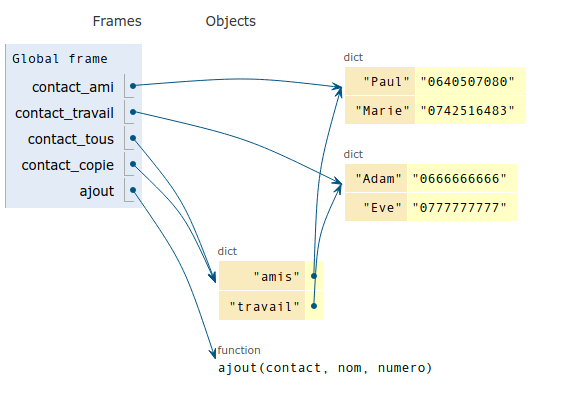
\includegraphics{images/attention.png}\\

\end{minipage} &

\begin{minipage}{0.5\linewidth}

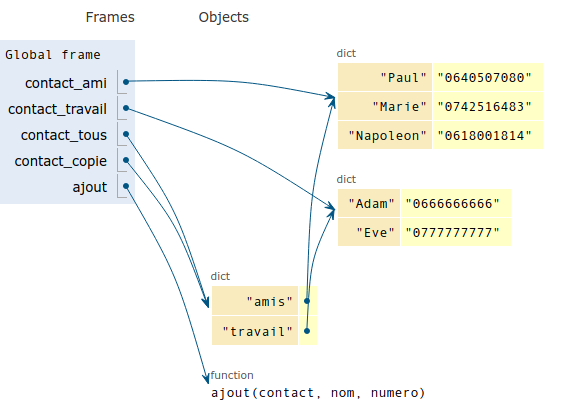
\includegraphics{images/attention2.png}\\

\end{minipage} \end{tabular}

\hypertarget{performance}{%
\section{Performance}\label{performance}}

\begin{propriete}{}

Les dictionnaires de type \passthrough{\lstinline!dict!} sont
implémentés en
\href{https://docs.python.org/3/tutorial/datastructures.html}{Python}
par des \href{https://fr.wikipedia.org/wiki/Table_de_hachage}{tables de
hachage} qui est une structure de données très efficace pour le test
d'appartenance, la recherche ou l'insertion d'élément. On peut
considérer que ces opérations se font en \textbf{temps quasiment
constant}, c'est-à-dire indépendant de la taille du dictionnaire alors
que la recherche et le test d'appartenance s'effectue en \textbf{temps
linéaire en moyenne} (proportionnel à la taille du tableau) pour les
tableaux de type \passthrough{\lstinline!list!} ou les
\passthrough{\lstinline!tuple!}. Cet optimisation des performances en
temps se fait au détriment de l'occupation en espace, les dictionnaires
étant plus gourmands en mémoire que les tableaux.

On donne ci-dessous un comparatif de temps d'exécutions pour la
recherche de 1000 flottants d'un tableau
\passthrough{\lstinline!needle!} (aiguilles) de taille 500, dans des
tableaux de flottants \passthrough{\lstinline!haystack!} (meule de foin)
de taille croissante \(10^{k}\) avec \(k \in \{3,4,5,6,7\}\). Pour
chaque test, les éléments de \passthrough{\lstinline!haystack!} et
\passthrough{\lstinline!needle!}sont tous distincts et la moitié de
\passthrough{\lstinline!needle!} est dans
\passthrough{\lstinline!haystack!}.

Le code de cet exemple, tiré de l'ouvrage Python Fluent de Luciano
Ramalho, est disponible avec nos commentaires dans l'archive
\href{https://gitlab.com/frederic-junier/nsi/-/blob/master/TypesConstruits/Dictionnaires/Cours/ressources/test_performance_in.zip}{test\_performance\_in.zip}.

\begin{lstlisting}
Type de conteneur dict
--------------------
Taille de la meule de foin :     1000
Temps minimum de recherche de 1000 aiguilles  (sur 5 recherches): 0.000104s
--------------------
Taille de la meule de foin :    10000
Temps minimum de recherche de 1000 aiguilles  (sur 5 recherches): 0.000196s
--------------------
Taille de la meule de foin :   100000
Temps minimum de recherche de 1000 aiguilles  (sur 5 recherches): 0.000252s
--------------------
Taille de la meule de foin :  1000000
Temps minimum de recherche de 1000 aiguilles  (sur 5 recherches): 0.000399s
--------------------
Taille de la meule de foin : 10000000
Temps minimum de recherche de 1000 aiguilles  (sur 5 recherches): 0.000483s
--------------------

Type de conteneur list
--------------------
Taille de la meule de foin :     1000
Temps minimum de recherche de 1000 aiguilles  (sur 5 recherches): 0.008002s
--------------------
Taille de la meule de foin :    10000
Temps minimum de recherche de 1000 aiguilles  (sur 5 recherches): 0.078902s
--------------------
Taille de la meule de foin :   100000
Temps minimum de recherche de 1000 aiguilles  (sur 5 recherches): 0.812977s
--------------------
Taille de la meule de foin :  1000000
Temps minimum de recherche de 1000 aiguilles  (sur 5 recherches): 8.554425s
--------------------
Taille de la meule de foin : 10000000
Temps minimum de recherche de 1000 aiguilles (sur 5 recherches):84.754335s
--------------------
\end{lstlisting}

\end{propriete}

\hypertarget{synthuxe8se}{%
\section{Synthèse}\label{synthuxe8se}}

\begin{memo}{}

\begin{itemize}
\tightlist
\item
  Le type construit \textbf{p-uplet nommé} est une séquence non ordonnée
  d'éléments qui sont des paires
  \passthrough{\lstinline!(clef, valeur)!} ou
  \passthrough{\lstinline!clef : valeur!}. Chaque
  \passthrough{\lstinline!valeur!} est indexée par sa
  \passthrough{\lstinline!clef!} et non par un index entier comme dans
  un \textbf{p-uplet}.
\item
  En
  \href{https://docs.python.org/3/tutorial/datastructures.html}{Python}
  un \textbf{p-uplet nommé} est un \textbf{dictionnaire} de type
  \passthrough{\lstinline!dict!} implémenté par une table de hachage qui
  permet des opérations très performantes en \textbf{temps constant}.
\item
  L'accès, l'ajout, la modification d'un dictionnaire s'effectue avec
  l'opérateur crochet et la syntaxe
  \passthrough{\lstinline!dico[clef] = valeur!}.
\item
  Une variable de type \passthrough{\lstinline!dict!} est une
  \textbf{référence} et elle peut être modifiée par effet de bord car
  c'est une valeur \textbf{mutable}.
\item
  Trois méthodes permettent le parcours de dictionnaire :

  \begin{itemize}
  \tightlist
  \item
    par clefs avec \passthrough{\lstinline!for clef in doc.keys()!}
  \item
    par valeurs avec \passthrough{\lstinline!for clef in doc.values()!}
  \item
    par paires \passthrough{\lstinline!(clef, valeur)!} avec
    \passthrough{\lstinline!for (clef, valeur) in doc.items()!}
  \end{itemize}
\end{itemize}

\end{memo}

\end{document}
